\documentclass[
  jou,
  floatsintext,
  longtable,
  nolmodern,
  notxfonts,
  notimes,
  colorlinks=true,linkcolor=blue,citecolor=blue,urlcolor=blue]{apa7}

\usepackage{amsmath}
\usepackage{amssymb}



\usepackage[bidi=default]{babel}
\babelprovide[main,import]{english}


% get rid of language-specific shorthands (see #6817):
\let\LanguageShortHands\languageshorthands
\def\languageshorthands#1{}

\RequirePackage{longtable}
\RequirePackage{threeparttablex}

\makeatletter
\renewcommand{\paragraph}{\@startsection{paragraph}{4}{\parindent}%
	{0\baselineskip \@plus 0.2ex \@minus 0.2ex}%
	{-.5em}%
	{\normalfont\normalsize\bfseries\typesectitle}}

\renewcommand{\subparagraph}[1]{\@startsection{subparagraph}{5}{0.5em}%
	{0\baselineskip \@plus 0.2ex \@minus 0.2ex}%
	{-\z@\relax}%
	{\normalfont\normalsize\bfseries\itshape\hspace{\parindent}{#1}\textit{\addperi}}{\relax}}
\makeatother




\usepackage{longtable, booktabs, multirow, multicol, colortbl, hhline, caption, array, float, xpatch}
\usepackage{subcaption}


\renewcommand\thesubfigure{\Alph{subfigure}}
\setcounter{topnumber}{2}
\setcounter{bottomnumber}{2}
\setcounter{totalnumber}{4}
\renewcommand{\topfraction}{0.85}
\renewcommand{\bottomfraction}{0.85}
\renewcommand{\textfraction}{0.15}
\renewcommand{\floatpagefraction}{0.7}

\usepackage{tcolorbox}
\tcbuselibrary{listings,theorems, breakable, skins}
\usepackage{fontawesome5}

\definecolor{quarto-callout-color}{HTML}{909090}
\definecolor{quarto-callout-note-color}{HTML}{0758E5}
\definecolor{quarto-callout-important-color}{HTML}{CC1914}
\definecolor{quarto-callout-warning-color}{HTML}{EB9113}
\definecolor{quarto-callout-tip-color}{HTML}{00A047}
\definecolor{quarto-callout-caution-color}{HTML}{FC5300}
\definecolor{quarto-callout-color-frame}{HTML}{ACACAC}
\definecolor{quarto-callout-note-color-frame}{HTML}{4582EC}
\definecolor{quarto-callout-important-color-frame}{HTML}{D9534F}
\definecolor{quarto-callout-warning-color-frame}{HTML}{F0AD4E}
\definecolor{quarto-callout-tip-color-frame}{HTML}{02B875}
\definecolor{quarto-callout-caution-color-frame}{HTML}{FD7E14}

%\newlength\Oldarrayrulewidth
%\newlength\Oldtabcolsep


\usepackage{hyperref}




\providecommand{\tightlist}{%
  \setlength{\itemsep}{0pt}\setlength{\parskip}{0pt}}
\usepackage{longtable,booktabs,array}
\usepackage{calc} % for calculating minipage widths
% Correct order of tables after \paragraph or \subparagraph
\usepackage{etoolbox}
\makeatletter
\patchcmd\longtable{\par}{\if@noskipsec\mbox{}\fi\par}{}{}
\makeatother
% Allow footnotes in longtable head/foot
\IfFileExists{footnotehyper.sty}{\usepackage{footnotehyper}}{\usepackage{footnote}}
\makesavenoteenv{longtable}

\usepackage{graphicx}
\makeatletter
\newsavebox\pandoc@box
\newcommand*\pandocbounded[1]{% scales image to fit in text height/width
  \sbox\pandoc@box{#1}%
  \Gscale@div\@tempa{\textheight}{\dimexpr\ht\pandoc@box+\dp\pandoc@box\relax}%
  \Gscale@div\@tempb{\linewidth}{\wd\pandoc@box}%
  \ifdim\@tempb\p@<\@tempa\p@\let\@tempa\@tempb\fi% select the smaller of both
  \ifdim\@tempa\p@<\p@\scalebox{\@tempa}{\usebox\pandoc@box}%
  \else\usebox{\pandoc@box}%
  \fi%
}
% Set default figure placement to htbp
\def\fps@figure{htbp}
\makeatother


% definitions for citeproc citations
\NewDocumentCommand\citeproctext{}{}
\NewDocumentCommand\citeproc{mm}{%
  \begingroup\def\citeproctext{#2}\cite{#1}\endgroup}
\makeatletter
 % allow citations to break across lines
 \let\@cite@ofmt\@firstofone
 % avoid brackets around text for \cite:
 \def\@biblabel#1{}
 \def\@cite#1#2{{#1\if@tempswa , #2\fi}}
\makeatother
\newlength{\cslhangindent}
\setlength{\cslhangindent}{1.5em}
\newlength{\csllabelwidth}
\setlength{\csllabelwidth}{3em}
\newenvironment{CSLReferences}[2] % #1 hanging-indent, #2 entry-spacing
 {\begin{list}{}{%
  \setlength{\itemindent}{0pt}
  \setlength{\leftmargin}{0pt}
  \setlength{\parsep}{0pt}
  % turn on hanging indent if param 1 is 1
  \ifodd #1
   \setlength{\leftmargin}{\cslhangindent}
   \setlength{\itemindent}{-1\cslhangindent}
  \fi
  % set entry spacing
  \setlength{\itemsep}{#2\baselineskip}}}
 {\end{list}}
\usepackage{calc}
\newcommand{\CSLBlock}[1]{\hfill\break\parbox[t]{\linewidth}{\strut\ignorespaces#1\strut}}
\newcommand{\CSLLeftMargin}[1]{\parbox[t]{\csllabelwidth}{\strut#1\strut}}
\newcommand{\CSLRightInline}[1]{\parbox[t]{\linewidth - \csllabelwidth}{\strut#1\strut}}
\newcommand{\CSLIndent}[1]{\hspace{\cslhangindent}#1}





\usepackage{newtx}

\defaultfontfeatures{Scale=MatchLowercase}
\defaultfontfeatures[\rmfamily]{Ligatures=TeX,Scale=1}





\title{Replication Project for the paper Immigration and Crime: An
International Perspective}


\shorttitle{Replication Project for the paper Immigration and Crime: An
International Perspective}


\usepackage{etoolbox}









\authorsnames{Yu-Chiao Tseng,Tawanda Nhundu}






\authorsaffiliations{
}




\leftheader{Tseng and Nhundu}



\abstract{This is a report of a replication study. Each group can freely
choose a research paper and try to interpret the code provided by the
author and replicate the charts with R.The replication process can be
assisted by ChatGPT and the file needs to be published on GitHub.This
report will cover all the steps to complete the report, the codes used
and the problems encountered during the replication. Although the
process was not always smooth, we managed to complete this report. }



\authornote{ 

\par{       }
\par{Correspondence concerning this article should be addressed
to Yu-Chiao
Tseng, Email: \href{mailto:tseng.yu-chiao@stud.hs-fresenius.de}{tseng.yu-chiao@stud.hs-fresenius.de}Tawanda
Nhundu, Email: \href{mailto:nhundu.tawanda@stud.hs-fresenius.de}{nhundu.tawanda@stud.hs-fresenius.de}}
}

\usepackage{pbalance}
% \usepackage{float}
\makeatletter
\let\oldtpt\ThreePartTable
\let\endoldtpt\endThreePartTable
\def\ThreePartTable{\@ifnextchar[\ThreePartTable@i \ThreePartTable@ii}
\def\ThreePartTable@i[#1]{\begin{figure}[!htbp]
\onecolumn
\begin{minipage}{0.485\textwidth}
\oldtpt[#1]
}
\def\ThreePartTable@ii{\begin{figure}[!htbp]
\onecolumn
\begin{minipage}{0.48\textwidth}
\oldtpt
}
\def\endThreePartTable{
\endoldtpt
\end{minipage}
\twocolumn
\end{figure}}
\makeatother


\makeatletter
\let\endoldlt\endlongtable		
\def\endlongtable{
\hline
\endoldlt}
\makeatother

\newenvironment{twocolumntable}% environment name
{% begin code
\begin{table*}[!htbp]%
\onecolumn%
}%
{%
\twocolumn%
\end{table*}%
}% end code

\urlstyle{same}



\makeatletter
\@ifpackageloaded{caption}{}{\usepackage{caption}}
\AtBeginDocument{%
\ifdefined\contentsname
  \renewcommand*\contentsname{Table of contents}
\else
  \newcommand\contentsname{Table of contents}
\fi
\ifdefined\listfigurename
  \renewcommand*\listfigurename{List of Figures}
\else
  \newcommand\listfigurename{List of Figures}
\fi
\ifdefined\listtablename
  \renewcommand*\listtablename{List of Tables}
\else
  \newcommand\listtablename{List of Tables}
\fi
\ifdefined\figurename
  \renewcommand*\figurename{Figure}
\else
  \newcommand\figurename{Figure}
\fi
\ifdefined\tablename
  \renewcommand*\tablename{Table}
\else
  \newcommand\tablename{Table}
\fi
}
\@ifpackageloaded{float}{}{\usepackage{float}}
\floatstyle{ruled}
\@ifundefined{c@chapter}{\newfloat{codelisting}{h}{lop}}{\newfloat{codelisting}{h}{lop}[chapter]}
\floatname{codelisting}{Listing}
\newcommand*\listoflistings{\listof{codelisting}{List of Listings}}
\makeatother
\makeatletter
\makeatother
\makeatletter
\@ifpackageloaded{caption}{}{\usepackage{caption}}
\@ifpackageloaded{subcaption}{}{\usepackage{subcaption}}
\makeatother

% From https://tex.stackexchange.com/a/645996/211326
%%% apa7 doesn't want to add appendix section titles in the toc
%%% let's make it do it
\makeatletter
\xpatchcmd{\appendix}
  {\par}
  {\addcontentsline{toc}{section}{\@currentlabelname}\par}
  {}{}
\makeatother

%% Disable longtable counter
%% https://tex.stackexchange.com/a/248395/211326

\usepackage{etoolbox}

\makeatletter
\patchcmd{\LT@caption}
  {\bgroup}
  {\bgroup\global\LTpatch@captiontrue}
  {}{}
\patchcmd{\longtable}
  {\par}
  {\par\global\LTpatch@captionfalse}
  {}{}
\apptocmd{\endlongtable}
  {\ifLTpatch@caption\else\addtocounter{table}{-1}\fi}
  {}{}
\newif\ifLTpatch@caption
\makeatother

\begin{document}

\maketitle




\setlength\LTleft{0pt}


\setcounter{page}{9}


\section{Introduction}\label{introduction}

The goal of this project is to conduct a replication study. Our group
selected the paper from Olivier Marie and Paolo Pinotti (2024) which
explored the association between immigration and crime in the Journal of
Economic Perspectives. They found that an increase in the share of
immigrants was not accompanied by an increase in the global murder rate.

We will discuss more detail the process of finding papers, how we used R
to complete this replication study, the challenges we encountered, and
how we published our report on GitHub. Lastly, we will summarize the
learning process.

\section{Motivation for Replication}\label{motivation-for-replication}

Academic research nowadays values transparency and credibility, and
replication studies are an important way to verify these.There are some
researchers manipulate data to achieve the results they want, and
replication studies can confirm that the author's research results are
not accidental or the result of incorrect analysis method. The
importance of research in science and academic knowledge is
self-evident. According to Bouter \& ter\,Riet (2021) replication is
divided into three different levels. First, reanalysis of the original
study by re‑running their exact code and dataset, to verify that the
published figures and tables can be fully reproduced. The second one is
direct replication which means replicate with new data but the same
research protocol. The third one is conceptual replication, researchers
use new data with the modified research protocol and same research
question. In the project I think we did re‑analysis, we used the data
provided by the authors and the same data analysis plan.Using the world
bank data as weight can be a conceptual replication. Bouter \& ter\,Riet
mentioned that by varying data sources or methods, conceptual
replications can reveal whether a finding can be use in different
context and proof it validity and generalizability. In contrast,
reanalyses or direct replications which rely on the same dataset or same
procedures might reproduce the flaws that were present in the original
study.

(\citeproc{ref-bouter2021a}{Bouter \& Riet, 2021})

\section{Finding a paper}\label{finding-a-paper}

We selected two papers, ``Inside the Box'' and ``Immigration and Crime''
at the beginning. The first one was written by an author who used R to
do most of his work, so the professor suggested that we choose another
one. In the article ``Immigration and Crime'', the author used Stata for
coding. The article explored the relationship between immigration and
crime. Living abroad as students, we felt that the increase in
immigration in many countries in recent years has brought benefits such
as filling the labor gap in developed countries, but it has also caused
many conflicts between immigrants and locals. Many people believe that
immigrants cause public security problems and have low tolerance for
them. Seeing this trend, enhanced our interest in this topic, and we
hope to learn more about the content of the article and how the author
conducts statistical analysis and explores this issue.

The authors Olivier Marie and Paolo Pinotti cleaned, merged, and
statistically analyzed the United Nations' immigration and crime data to
explore whether there is a significant correlation between immigration
and crime. They also referred to other studies to further explore
whether obtaining legal status reduces the tendency to commit crimes. We
chose Figure 2 and Figure 4 for replication. First, we read the author's
README file and Stata code to confirm the feasibility and verify whether
the data set can be accessed from the websites they provided.

\section{Figure 2 Top Replication
Process}\label{figure-2-top-replication-process}

Figure 2 is composed of two figures, the first one is a double y-axis
graph, showing the long-term trend of the ``proportion of immigrants to
the total population'' gray line and the ``murder rate'' blue line in 55
countries (1990-2019). The second figure is a scatter plot, showing how
much the ``number of immigrants'' in each country changed from 1990 to
2019 and how much the ``murder rate'' changed during the same period
(calculated in logarithms).

\phantomsection\label{fig:original}
\textbf{Figure~1.}\\
\emph{Original graph of Figure~2}

\begin{center}
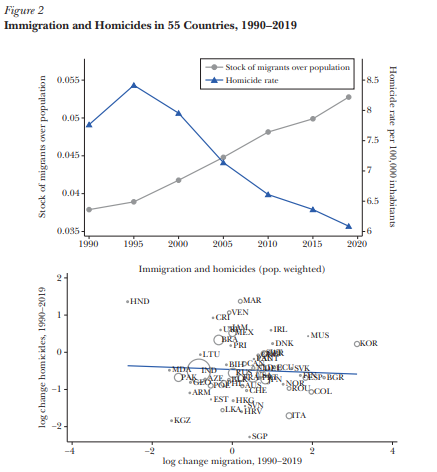
\includegraphics[width=0.8\linewidth,height=\textheight,keepaspectratio]{fig/Original.png}
\end{center}

(\citeproc{ref-marie2024}{Marie \& Pinotti, 2024})

Below is the original Stata code for Figure 2 top

\phantomsection\label{fig:statatop}
\textbf{Figure~2.}\\
\emph{Original Stata code Figure 2 top}

\begin{center}
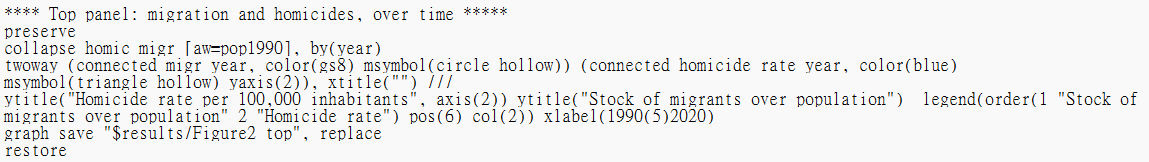
\includegraphics[width=0.8\linewidth,height=\textheight,keepaspectratio]{fig/statatop.png}
\end{center}

This part I relied on chatgpt's explanation to understand the meaning of
each code collapse homic migr {[}aw=pop1990{]}, by(year) is grouped by
year, and the variables homic and migr are weighted averaged (weight is
pop1990), Two-way connected plot is a two-line graph, connected migr
year, color(gs8) msymbol(circle\_hollow) draws the first line (left Y
axis), connected homicide\_rate year, color(blue)
msymbol(triangle\_hollow) yaxis(2) draws the second line (right Y axis).
Then I created a new file in R and saved the data provided by the
author. ChatGPT guided me step by step to reproduce this grpah in R.

(OpenAI, 2025)

Here is the first problem. As we can see, the gray line on the graph
made according to the above code is almost attached to the bottom of the
graph. I asked Chatgpt, and it said that the gray ``immigrant
proportion'' line is always close to 0. This is because the dual Y axes
of ggplot2 are not truly ``independently scaled'', but share a set of
numerical spaces. hom\_w (murder rate) is about 6 to 9, and migr\_w
(immigrant proportion) is about 0.03 to 0.055. After looking at the
graph, I also noticed that the scales on both sides of my graph are 0-8,
while the scale on the left side of the author's graph is 0.035-0.055.

Then ChatGPT Offered Solution:

\phantomsection\label{fig:S2}
\textbf{Figure~3.}\\
\emph{Solution for flat gray line}

\begin{center}
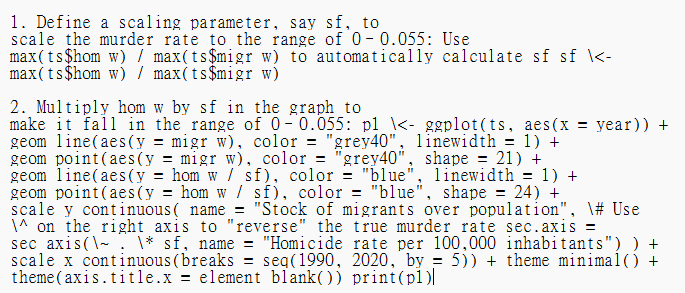
\includegraphics[width=0.8\linewidth,height=\textheight,keepaspectratio]{fig/S2.png}
\end{center}

(OpenAI, 2025)

Here I follow the instruction, use y = hom\_w / sf when drawing the blue
line (equivalent to ``compressing'' the murder rate to the small
interval of the proportion of immigrants), Then use
sec\_axis(\textasciitilde{} . * sf) to ``expand'' the label on the right
back to the true murder rate value. After following the steps of
chatgpt, the two lines are in the correct position. Lastly, I corrected
the scales on both sides to 0.035-0.055 on the left axis and 6-8.5 on
the right axis.

After following the steps of ChatGPT, the two lines are now in the
correct position. Lastly, I corrected the scales on both sides to
0.035-0.055 on the left axis and 6-8.5 on the right axis to make it more
alike to original one.

I also noticed that the gray line ended up closer to 8.5, while the
original graph looked between 8 and 8.5. I asked ChatGPT and checked
three things according to it's instructions. 1. Did I draw 2020 ? 2.
Confirm that migr\_pop is a proportion, not a number of people 3.
Re-ensure that the weighted average uses the pop1990 column I checked
all of them, but the graph did not change. ChatGPT said that it might be
that the weighting method in Stata is slightly different from the
implementation details in R, or that the original graph was slightly
adjusted manually when it was published.(OpenAI, 2025) I remember
learning in the course last semester that the key to doing replication
is to be able to reproduce the results and trends that the chart wants
to present after following the code provided by the author and the same
method. In this graph, the direction of the lines is consistent with the
changes (immigration increased, murders decreased), and the values are
roughly in the same area, with no obvious misalignment or data errors. I
think the points where the two lines fall and where they intersect are
not significantly different from the original graph, so I believe this
is a successful replication.

\subsection{Discussion on Figure 2
top}\label{discussion-on-figure-2-top}

Figure 2 top graph uses United Nations immigration data. I think the
author could be more precise on that. Did they use International migrant
stock from United Nations data or Total population, or both? At first, I
compared the numbers on the data and the website, and found that there
was a slight difference between the total population on the website and
the file provided by the author. For example, the total population of
Australia in 1990 was 16960.600 in the author's data and 17126.298 on
the website. The total population of Armenia in 1990 was 3538.164, and
3552.128 on the website. I thought that this might be because the data
on the website had been updated. If the difference was not big, I
thought the data provided by the author was credible, so I directly used
the author's data for replication. Later, I further wanted to confirm
where the number of migr\_pop in the author's file came from, but I
couldn't calculate a similar number. Finally, I realized the problem is
that I downloaded the latest version of the data, and the author used
the 2020 version. The latest version is Armenia 1990 Total population at
mid-year 3552.128, migrant stock 433541. The version used by the author,
Armenia 1990 Total population at mid-year 3538.164, migrant stock has
been updated a lot, which led to my calculation of 433541/3552.128
≈0.1225, not ≈0.186. Another issue was the numbers for migrant stock are
missing from the file provided by the authors; it has only the author's
own calculation of migr\_pop 0.186195165. I think the author's readme
file can include the file year used and how migr\_pop is calculated.
This can improve the overall transparency and credibility of the
research and reduce disputes over errors caused by different versions.

\section{Figure 2 Bottom Replication
Process}\label{figure-2-bottom-replication-process}

The bottom plot is the logarithmic change scatter plot + weighted
regression line for 1990 vs.~2019. X axis: log change migration, Y axis:
log change homicides

Below is the original Stata code for Figure 2

\phantomsection\label{fig:statabottom}
\textbf{Figure~4.}\\
\emph{original Stata code Figure 2 bottom}

\begin{center}
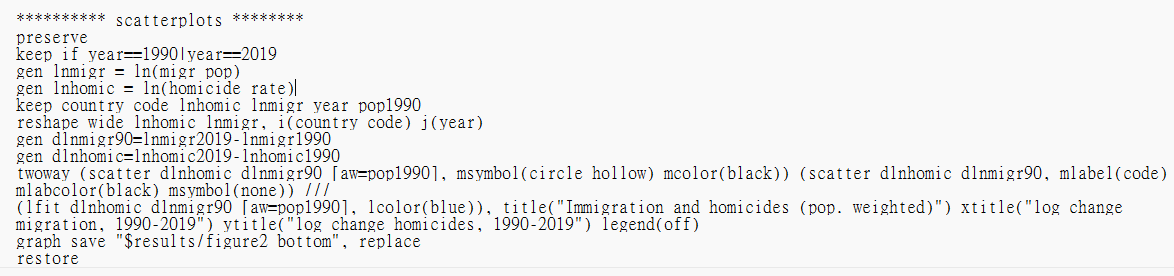
\includegraphics[width=0.8\linewidth,height=\textheight,keepaspectratio]{fig/statabottom.png}
\end{center}

Same I followed the instructions of ChatGPT to do the steps, first
select 1990 and 2019 from the original data

It looks very similar to the original image, and then I adjusted the
scale.

Lastly, I use the code theme\_minimal(base\_size = 38) for the font size
adjustment. I think this graph shares the same idea that the author
wants to present in the paper. There is a nearly horizontal regression
line, and most countries are concentrated between -1 and 1 on the X
axis. This means that the proportion of immigrants and the murder rate
in most countries have not experienced a huge change. If more immigrants
lead to higher crime, there will be a cluster in the upper right corner
of the graph. However, the graph shows that there is no consistent trend
or causal relationship between changes in immigration and changes in
murder rates.

\section{Using World Bank population data as
weight}\label{using-world-bank-population-data-as-weight}

Because the group before us had some data generation problems, they
didn't seem to use the data used by the author, but the graph was
produced. The professor said that their data might be generated by
ChatGPT itself, and then said that they could go to the World Bank to
find the data they needed. At that time, I thought I had to use the
World Bank data, so I used the World Bank data to make the second graph.
But I didn't give ChatGPT instructions clear enough; I just said that I
wanted to use the World Bank population data to make a new graph.So
ChatGPT gave me the code:

The step after merging had mistake

\phantomsection\label{fig:M1}
\textbf{Figure~5.}\\
\emph{Mistake using incorrect weights}

\begin{center}
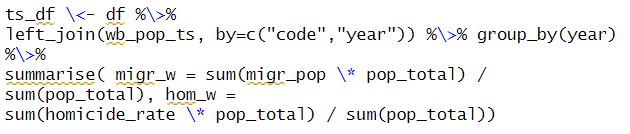
\includegraphics[width=0.8\linewidth,height=\textheight,keepaspectratio]{fig/M1.png}
\end{center}
Because I used the total population of all years from 1990 to 2019, what
I got was the ``weighted average of the population distribution of that
year'', which means that the weights change every year. Actually, I
don't need the total population of all years from 1990 to 2019. I only
need to replace the 1990 population (pop1990) with World Bank's data,
because the author used only the 1990 population (pop1990) as the weight
for all periods.

Second time, I only used the 1990 population as the weight for the whole
period, and I still use the migr\_pop calculated by the author as a
share.

\subsection{Discussion of using the data from the World Bank
incorrectly}\label{discussion-of-using-the-data-from-the-world-bank-incorrectly}

This graph looks very different from the last graph with mistakes, and
doesn't look significantly different from the first time I used the data
provided by the author.

This time, I used the data from the World Bank incorrectly and didn't
notice it at all. I intuitively thought that the graph looked different
only because I used the data from the World Bank. This caused me to be
embarrassed during my oral presentation.

\subsection{Problems with making a scatter plot at the
bottom}\label{problems-with-making-a-scatter-plot-at-the-bottom}

I also tried to make the bottom plot using the data from the World Bank,
but the problem I had was scatter plots did not appear.

I asked ChatGPT why this code can't make a scatter plot; the plot is
blank, there is no dots. At first, it couldn't find the reason, and
ChatGPT kept going around in circles. After hours, I changed the
conversation to a new chat room and re-posted the code. It finally works
and I just checked it step by step according to its instructions. For
example, check whether there are rows in the final data frame before
drawing, and checked which countries are not in wb\_pop.

Finally, we found the problem, and ChatGPT explained it this way: The
problem is in the plot data frame, all rows corresponding to x =
dln\_migr or y = dln\_homic are treated as NA, so ggplot automatically
discards them.

The solution provided from ChatGPT is to keep only the columns I need
before pivoting

\phantomsection\label{fig:S1}
\textbf{Figure~4.}\\
\emph{Solution for blank scatter plot}

\begin{center}
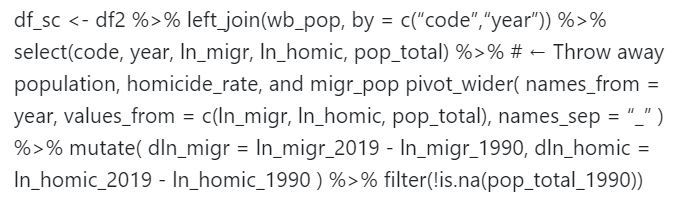
\includegraphics[width=0.8\linewidth,height=\textheight,keepaspectratio]{fig/S1.png}
\end{center}

(OpenAI, 2025)

After correcting according to the instructions, the scattered points
appeared.

\section{Conclusion Summarizing}\label{conclusion-summarizing}

Through this replication process and the professor's explanation in
class, I understand the importance of replication for research. It not
only confirms the transparency and credibility of the research, can also
checks whether there are errors or artificial manipulation of data in
the analysis process. The first time I used all the data provided by the
author to make the chart, and only compared the numbers on the website
with the file. The second time I used the data from the World Bank,
although it was under a misunderstanding of the discussion in class,
which resulted in many errors, but on the other hand taught me a lot.

Honestly, after the presentation, I still don't know if it makes sense
for me to use the data from the World Bank, cause I still use the
original calculation of migr\_pop by the author. I asked ChatGPT, and
its answer was: ``If the purpose of your research is just want to see
what happens if you use the WDI population as weight, then it makes
sense to do so: it can answer a new question: If I use the World Bank's
1990 population as weight instead, how will the trend of the global
immigrant share be fine-tuned? This may also be an interesting
robustness check in policy or methodological discussions.'' Seeing the
answer, I was glad that it was not a waste of time. Although using the
World Bank data may not help replicate the graph itself, it's meaningful
to the learning process, and it allowed me to learn how to add the World
Bank data in R and use it correctly.

If I hadn't taken this class, I would have never thought about learning
how to use R or how to write code. I often couldn't understand what the
professor was doing in class, I felt lost in the lecture or I forgott
what to do after Professor finished demonstrating. It started changing
until I had to make this Replication report. At the beginning I did
everything slowly, and when R shows that I had error, I didn't know what
happened. I had to take screenshot and sent it to ChatGPT.Under the
guidance of ChatGPT, I was able to create the graph step by step.
Although I still made a lot of mistakes like the first time I tried to
replicate the graph, I put all the code into the console, and it
worked,the graph showed, but I was not able to keep the code for the
report. When modifying some part of the code, I also made mistakes such
as missing a ) or missing a comma, adding an extra comma, and made an
Incorrect data path etc.Some of the mistakes took me a lot of time to
figure the problems out and fixed them.Lack of familiarity with R often
slows down our progress and was very frustrating.

After I learnt how to create graphs, I even used R to create more graphs
in another group project, which was something I had never expected at
the beginning of the semester, and I am proud of my learning process.

\phantomsection\label{fig:dhl}
\textbf{Figure~6.}\\
\emph{Graph for DHL Project created with R}

\begin{center}
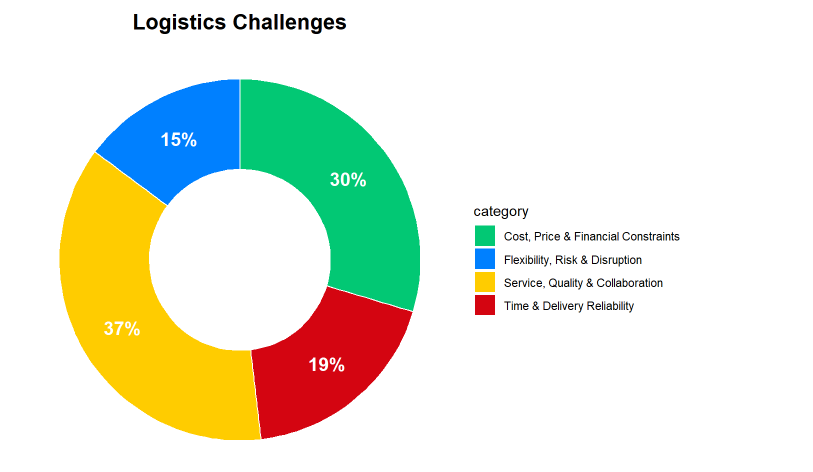
\includegraphics[width=0.8\linewidth,height=\textheight,keepaspectratio]{fig/dhl.png}
\end{center}

\section{Limitations and Future
Directions}\label{limitations-and-future-directions}

The Limitations of this report, we only found data that the author had
cleaned up, which contained the migr\_pop calculated by the authors. We
only compared the total population and murder rate provided by the
authors with the numbers on the websites, and did not download the
original data of these two catagories and recalculate migr\_pop to
verify the numbers provided by the authors.

I think the further direction of this replication study could be to
first use the latest version of immigration data on the UN website for
Figure 2. As I mentioned earlier, the numbers of migration stock are
quite different from the previous version. However, this would involve
recalculating migr\_pop ourselves. second, other violent crimes can also
be included to re-examine the relationship between immigration and crime
rates. Third, use the same analysis method to explore different cities
in a certain country.

\section{References}\label{references}

\phantomsection\label{refs}
\begin{CSLReferences}{1}{0}
\bibitem[\citeproctext]{ref-bouter2021a}
Bouter, L. M., \& Riet, G. ter. (2021). Replication Research
Series-Paper 2 : Empirical research must be replicated before its
findings can be trusted. \emph{Journal of Clinical Epidemiology},
\emph{129}, 188--190.
\url{https://doi.org/10.1016/j.jclinepi.2020.09.032}

\bibitem[\citeproctext]{ref-marie2024}
Marie, O., \& Pinotti, P. (2024). Immigration and Crime: An
International Perspective. \emph{Journal of Economic Perspectives},
\emph{38}(1), 181--200. \url{https://doi.org/10.1257/jep.38.1.181}

\end{CSLReferences}

OpenAI. (2025). ChatGPT {[}Large language model{]}.
https://chat.openai.com/chat

\appendix

\section{}\label{}

\section{}\label{apx-a}






\end{document}
